\documentclass[a4paper,12pt]{article} % добавить leqno в [] для нумерации слева
\usepackage[a4paper,top=1.3cm,bottom=2cm,left=1.5cm,right=1.5cm,marginparwidth=0.75cm]{geometry}
%%% Работа с русским языком
\usepackage{cmap}					% поиск в PDF
\usepackage[warn]{mathtext} 		% русские буквы в фомулах
\usepackage[T2A]{fontenc}			% кодировка
\usepackage[utf8]{inputenc}			% кодировка исходного текста
\usepackage[english,russian]{babel}	% локализация и переносы
\usepackage{multirow}
\usepackage{float}
\restylefloat{table}


\usepackage{graphicx}

\usepackage{wrapfig}
\usepackage{tabularx}

\usepackage{hyperref}
\usepackage[rgb]{xcolor}
\hypersetup{
	colorlinks=true,urlcolor=blue
}

%%% Дополнительная работа с математикой
\usepackage{amsmath,amsfonts,amssymb,amsthm,mathtools} % AMS
\usepackage{icomma} % "Умная" запятая: $0,2$ --- число, $0, 2$ --- перечисление

%% Номера формул
\mathtoolsset{showonlyrefs=true} % Показывать номера только у тех формул, на которые есть \eqref{} в тексте.

%% Шрифты
\usepackage{euscript}	 % Шрифт Евклид
\usepackage{mathrsfs} % Красивый матшрифт

%% Свои команды
\DeclareMathOperator{\sgn}{\mathop{sgn}}

%% Перенос знаков в формулах (по Львовскому)
\newcommand*{\hm}[1]{#1\nobreak\discretionary{}
	{\hbox{$\mathsurround=0pt #1$}}{}}

\date{\today}

\begin{document}

	{\huge
		\begin{center}
			{\bf Отчёт о выполнении лабораторной работы 1.1.6}\\
			Изучение электронного осциллографа
		\end{center}
	}

	\section{Аннотация}
	
	\textbf{Цель работы:} ознакомиться с устройством и работой осциллографа. научиться измерять ам- плитуды и частоты произвольных сигналов; изучить основные характеристики осциллографа и их влияние на искажение сигналов.\\
	\textbf{В работе используются:} осциллограф \textit{GWINSTEK GOS-620}, генераторы электрических сигналов, соединительные кабели.
	
	\section{Теоретические сведения}
	
	Осциллограф - регистрирующий прибор, в котором исследуемое напряжение (сигнал) преобразуется в видимый на экране график изменения напряжения во времени. Осциллограф широко используется в физическом эксперименте. С его помощью можно исследовать изменение во времени любых физических величин, которые могут быть преобразованы в электрические сигналы.
	
	\begin{wrapfigure}{r}{10cm}
		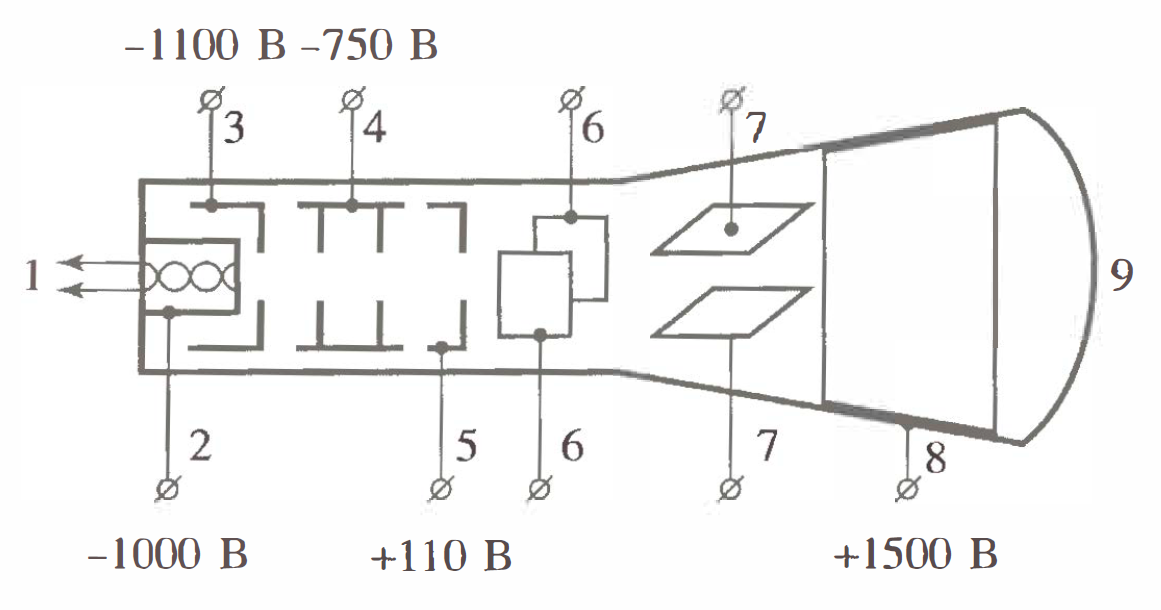
\includegraphics[width=10cm]{truba.png}
		\caption{Электронно-лучевая трубка}
		\label{ELT}
	\end{wrapfigure}
	
	На рис. \ref{ELT} показано устройство основной части электронного осциллографа -- электронно-лучевой трубки. Трубка представляет собой откачанную до высокого вакуума колбу, в которой расположены: подогреватель катода \textbf{1}, катод \textbf{2}, модулятор \textbf{3} (электрод, управляющий яркостью изображения), первый (фокусирующий) анод \textbf{4}, второй (ускоряющий) анод \textbf{5}, горизонтально и вертикально отклоняющие пластины \textbf{6} и \textbf{7}, третий (ускоряющий) анод \textbf{8}, экран \textbf{9}. 
	
	При наблюдении периодических и особенно быстропротекающих процессов важно получить на экране осциллографа неподвижное изображение сигнала. 
	Для этого нужно, чтобы период развертки был кратен периоду изучаемого сигнала. Однако, как правило, точное соотношение периодов соблюсти трудно из-за нестабильности генератора развертки или самого изучаемого процесса.
	Поэтому используют принудительное согласование периодов, при котором изучаемое напряжение «навязывает» свой период генератору развертки. При этом начало прямого хода развёртки должно совпадать строго с одной и той же характерной точкой исследуемого периодического сигнала. 
	Процесс привязки начала развертки к характерным точкам сигнала называется \textit{синхронизацией} развертки с сигналом.
	
	В процессе работы с осциллографом всегда следует учитывать частотные характеристики каналов вертикального и горизонтального отклонения: амплитудно-частотную характеристику (АЧХ) и фазо-­частотную характеристику (ФЧХ). Если на вход <<Y>> осциллографа подаётся синусоидальное напряжение $ U_y=U_0\sin\left(2\pi ft\right) $ амплитудой $ U_0 $ и частотой $ f $, то для перемещения луча на экране ЭЛТ можно записать: $ y=y_0\left(f\right)\sin\left(2\pi ft + \Delta\Phi_y\left(f\right)\right) $. Здесь $ U_0 $ -- амплитуда перемещения луча на частоте $ f $, $ \Delta\Phi_y\left(f\right) $ - разность между фазой колебаний перемещения луча $ y $ и фазой колебаний входного сигнала $ U_y $ на частоте $ f $ (сдвиг фаз).
	
	Тогда АЧХ канала вертикального отклонения есть зависимость:
	
	\begin{equation}
		K_y\left(f\right) = \frac{y_0\left(f\right)}{U_0}, \label{ahch}
	\end{equation}
	а ФЧХ - зависимость $ \Delta\Phi_y\left(f\right) $.
	
	При сложении двух взаимно перпендикулярных колебаний с равными или кратными частотами, поданных на входы осциллографа, луч описывает на экране неподвижные замкнутые кривые, которые называются \textbf{фигурами Лиссажу}. При небольшом нарушении кратности частот форма фигур медленно меняется, а при большом - картина размывается.
	
	Фигура, которую описывает луч при сложении колебаний, имеющих одинаковую частоту, представляет собой эллипс. Ориентация этого эллипса зависит от разности фаз колебаний $ \left(\varphi_2-\varphi_1\right) $.
	
	\begin{wrapfigure}{r}{10cm}
		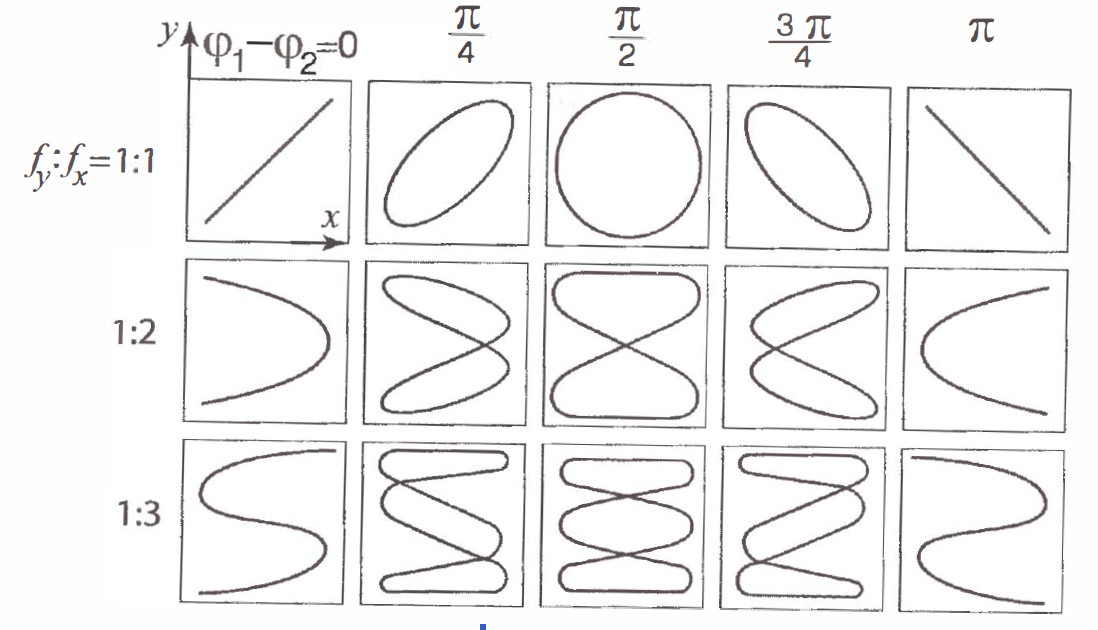
\includegraphics[width=10cm]{l_prim.png}
		\caption{Фигуры Лиссажу для колебаний одинаковой амплитуды}
		\label{l_prim}
	\end{wrapfigure}
	
	В общем случае вид фигуры Лиссажу зависит от соотношений между периодами (частотами), фазами и амплитудами складываемых колебаний. Некоторые частные случаи фигур Лиссажу для разных периодов и фаз показаны на рис. \ref{l_prim}. Зная параметры одного колебания, 
	например $ f_x $, можно по фигуре Лиссажу определить параметры другого колебания -- $ f_y $. На полученное изображение накладывают мысленно две линии -- горизонтальную и вертикальную, не проходящие через узлы фигуры. Фиксируют число пересечений с горизонтальной линией $ n_x $ и вертикальной линией $ n_y $ . Отношение частот $ f_y/f_x $ равно отношению $ n_x/n_y $. 
	

	\section{Методика измерений}
	\subsection{Подготовка}
	\begin{enumerate}
		\item    Блок горизонтальной развертки (HORIZONTAL): ручка POSITION -  в среднем положении; кнопка х10 MAG - отжата; ручка SWP.VAR - в крайнем правом положении;
		\item    Блок вертикального отклонения (VERTICAL): ручки POSITION — в среднем положении; внешние ручки VOLTS/DIV обоих каналов в положении 5 V/дел, а внутренние — утоплены; тумблеры AC–GND–DC обоих каналов — в положении GND (отключены); кнопки ALT/CHOP и INV CH 2 — отжаты.
		\item    Блок синхронизации (TRIGGER): TRIG.ALT — отжата, LEVEL — в среднем положении; переключатель MODE — в положении AUTO; SLOPE — отжата.
		\item    Включаем осциллограф в сеть. Ставим ручку развертки
		TIME/DIV в положение X–Y. На экране появится точка. Ручками POSITION располагаем точку в центре экрана осциллографа. Регулируем яркость и четкость изображения точки ручками INTEN и FOCUS — размер и яркость точки должны быть минимально возможными, при условии, что точка хорошо видна на экране. После регулировки включите внутреннюю развертку осциллографа, установив ручку TIME/DIV в положение 2 ms.	
	\end{enumerate}
	\subsection{Наблюдение периодического сигнала и измерение его частоты.}
	\begin{enumerate}
		\item Подключите звуковой генератор к каналу «CH2(Y)» и настройте
		его на синусоидальный сигнал некоторой не слишком высокой частоты
		(например, $f \approx$ 1 кГц).
		\item Убедитесь, что тумблер MODE блока
		VERTICAL и тумблер SOURCE блока «TRIGGER» находятся
		в положении «CH2(Y)». Установите режим открытого (DC) входа
		для канала «CH2(Y)».
		\item Получите на осциллографе устойчивую картину колебаний. \\
		Используйте ручки «VOLTS/DIV» (вольт/деление)
		для регулировки масштаба по вертикали, ручку «TIME/DIV» (время/деление)
		для регулировки масштаба по горизонтали, и ручки «POSITION»
		для смещения картины как целого. Настройте уровень запуска развёртки (ручка «LEVEL») для получения стационарной картины.
		При необходимости переключайте режим синхронизации тумблером «MODE» блока «TRIGGER» в положения «AUTO» (автоматический режим) или «NORM» (режим ожидания).
		\item Измерьте период наблюдаемого сигнала $T$ (с учётом масштаба по горизонтальной оси, определяемого положением ручки
		«TIME/DIV») и найдите его частоту $f$ = $1/T$. Оцените минимальную относительную погрешность измерения периода $\delta T / T$ с помощью шкалы на экране осциллографа. Вычислите абсолютную погрешность определения частоты $\delta f = f\delta T /T$. Сравните результаты
		измерений с показанием $\nu_{\text{ЗГ}}$ встроенного в генератор частотомера.
		\item Повторите измерения для 5—7 различных частот из всего диапазона работы звукового генератора. Результаты занесите в таблицу.
	\end{enumerate}
	\subsection{Измерение амплитуды сигнала}
С помощью вертикальной шкалы экрана осциллографа измерьте несколько значений амплитуды сигнала от звукового генератора при различном положении его
ручек регулировки. В качестве примера предлагается измерить максимальную и минимальную амплитуды напряжений $U_{max}$, $U_{min}$, которые способен выдавать генератор, а также несколько промежуточных
значений. Измерения проведите на частоте $f = 1$ кГц.
	\begin{enumerate}
		\item Установите «AMPL» генератора
		сигналов на максимум (по часовой стрелке до упора). Убедитесь,
		что ручка не вытянута на себя, а кнопка «ATT -20dB»
		не нажата. С помощью осциллографа измерьте максимальную амплитуду генерируемого сигнала $U_{max}$.
		\item Нажмите на генераторе кнопку кнопку «ATT -20dB» (ослабление
		на 20 дБ - т. е. уменьшение амплитуды в 10 раз). Измерьте получившееся значение амплитуды $U_{-20dB}$. Вытяните ручку «AMPL» на себя (дополнительное ослабление на 20 дБ) и снова
		измерьте получившуюся амплитуду ($U_{-40dB}$). Наконец, установите минимально возможную амплитуду генератора, повернув ручку «AMPL» против часовой стрелки до упора. Измерьте величину
		$U_{min}$.
		Для изменения масштаба вертикальной шкалы осциллографа используйте ручку VOLTS/DIV (вольт на деление) канала
		CH2(Y). При измерении убедитесь, что серая ручка плавной регулировки VOLTS/DIV утоплена и переведена в крайнее правое
		положение до щелчка.
		\item Оцените абсолютную $\delta U$ и относительную $\delta U/U$ погрешности измерения амплитуды.
		\item Выразите отношения амплитуд измеренных сигналов
		\[(U_{max}/U_{-20dB}, U_{-20dB}/U_{-40dB}, U_{-40dB}/U_{min})\] в децибелах [дБ].
		Сравните получившиеся значения с расчётными.
	\end{enumerate}
	\section{Используемое оборудование}
	Погрешность осциллографа для прямого измерения периода сигнала $ \delta T $ равна половине цены малого деления осциллографа, т.е. $ \frac{1}{10} $ части от TIME/DIV.

	\section{Результаты измерений и обработка данных}
	
	\subsection{Наблюдение периодического сигнала от генератора и измерение его частоты}
	
	Получим на экране осциллографа устойчивую картину периодического (синусоидального) сигнала, подаваемого с генератора, и с помощью горизонтальной шкалы экрана осциллографа проведём измерение периода и частоты сигнала. Полученные результаты занесём в таблицу.
	
	\begin{table}[H]
		\centering
		\caption{Определение частоты сигнала при помощи осциллографа}
		\begin{tabular}{|c|c|c|c|c|c|c|c|c|c|}
			\hline
			№ & $ \nu_\text{ЗГ} $,Гц & $ T' $,~дел & TIME/DIV,мс & $ T $,мс & $ \delta T $,мс & $ \varepsilon_T $, \% & $ \nu_\text{изм} $,Гц & $ \delta f $,Гц & $ \left| \nu_\text{ЗГ} - \nu_\text{изм} \right| $,Гц \\ \hline
			1 &  &  &  &  &  &  &  &  &  \\ \hline
			2 &  &  &  &  &  &  &  &  &  \\ \hline
			3 &  &  &  &  &  &  &  &  &  \\ \hline
			4 &  &  &  &  &  &  &  &  &  \\ \hline
			5 &  &  &  &  &  &  &  &  &  \\ \hline
			6 &  &  &  &  &  &  &  &  &  \\ \hline
		\end{tabular}
		\label{tab:chastota}
	\end{table}
	
	
	Частоту сигнала можно вычислить по следующей формуле:
	
	\begin{equation}
		f_\text{изм} = \frac{1}{T}.
	\end{equation}
	
	Тогда погрешность вычисления $ f_\text{изм} $ равна:
	
	\begin{equation}
		\delta f_\text{изм} = f_\text{изм}\varepsilon_T.
	\end{equation}
	Полученные данные заносим в таблицу \ref{tab:chastota}.
	
	\subsection{Измерение амплитуды сигнала}
	
	С помощью вертикальной шкалы осциллографа проведём измерение амплитуды сигнала. Для этого установим значение частоты входного сигнала осциллографа 1 кГц, затем измерим отношение $ \frac{U_{max}}{U_{-20db}} $, $ \frac{U_{-20db}}{U_{-40db}} , \frac{U_{-40db}}{U_{min}}$, которые способен выдавать генератор. Результаты измерений занесем  таблицу \ref{tab:my-table}
	
	\begin{table}[H]
		\centering
		\begin{tabular}{|p{2.1cm}|p{2.1cm}|p{2.1cm}|p{2.1cm}|p{2.1cm}|c|c|c|c|c|c|}
			\hline
			$ U_{max} $, В & $ \delta U_{max} $, В & $ \varepsilon_{U_{max}} $, \% & $ U_{min} $, В & $ \delta U_{min} $, В & $ \varepsilon_{U_{min}} $, \% \\ \hline
			 & &  &  &  &   \\ \hline
		\end{tabular}
	\end{table}	
	\vspace{-1cm}
	\begin{table}[H]
		\centering
		\begin{tabular}{|p{2cm}|p{2cm}|p{2cm}|p{2cm}|p{2cm}|c|c|c|c|c|c|}
			\hline
			$ U_{-20db} $, В & $ \delta U_{-20db} $, В & $ \varepsilon_{U_{-20db}} $, \% & $ U_{-40db} $, В & $ \delta U_{-40db} $, В & $ \varepsilon_{U_{-40db}} $, \% \\ \hline
			& &  &  &  &   \\ \hline
		\end{tabular}
		\caption{Измерение амплитуды сигнала}
		\label{tab:my-table}
	\end{table}	
	\newpage
	
	\subsection{Наблюдение фигур Лиссажу}
	
	Для наблюдения фигур Лиссажу необходимо подать на 2 входа осциллографа 2 	сигнала различной частоты, причём их частоты должны соотноситься, как целые числа. После получения устойчивой картины фигуры Лиссажу, с помощью изображения можно определить соотношение частот входных сигналов. Для определения соотношения необходимо провести 2 произвольные линии, параллельные осям и не пересекающие фигуру в узловых точках, затем посчитать колличество точек пересечения данных прямых с фигурой. Отношение этих чисел -- есть искомое соотношение между частотами.			
	
	
	\subsection{Измерение амплитудно-частотной характеристики осциллографа}
	
	Амплитудо-частотной характеристикой (АЧХ) измерительного прибора называют зависимость амплитуды измеряемого
	сигнала от частоты сигнала, подаваемого на вход. Проведём измерение АЧХ используемого в работе осциллографа во всём диапазоне
	рабочих частот генератора по формуле \eqref{ahch}.
	
	Результаты измерений занесём в таблицу \ref{tab:ahch}.
	
	\begin{table}[H]
		\centering
		\begin{tabular}{|c|p{1.2cm}|p{1.2cm}|p{1.2cm}|p{1.2cm}|p{1.2cm}|p{1.2cm}| c|c|c|c|c|c|c|} 
			\hline
			№ &  1  & 2  &  3  &  4  & 5 & 6 \\ \hline
			$ f $, Гц &   &  &  &  & &  \\ \hline
			$ \lg f $ &  &  &  &  & &  \\ \hline
			$ 2U_{AC} $, дел & &  &  &  & &  \\ \hline
			$ K_{AC} = \frac{U_{AC}}{U_0} $& &  &  &  & &  \\ \hline
			$ 2U_{DC} $, дел & &  &  &  & &  \\ \hline
			$ K_{DC} = \frac{U_{DC}}{U_0} $ & &  &  &  & &  \\ \hline \hline
			№ & 7 & 8 & 9 & 10 & 11 & 12 \\ \hline
			$ f $, Гц & &  &  &  & &  \\ \hline
			$ \lg f $ & &  &  &  & &  \\ \hline
			$ 2U_{AC} $, дел & &  &  &  & &  \\ \hline
			$ K_{AC} = \frac{U_{AC}}{U_0} $ & &  &  &  & &  \\ \hline
			$ 2U_{DC} $, дел & &  &  &  & &  \\ \hline
			$ K_{DC} = \frac{U_{DC}}{U_0} $ & &  &  &  & &  \\ \hline
		\end{tabular}
		\caption{Измерение АХЧ осциллографа}
		\label{tab:ahch}
	\end{table}
	
	Причиной различия АХЧ осциллографа в разных режимах работы является ёмкость, включающаяся в схему осциллографа в режиме AC. При больших частотах её влияние становится мало, и оно почти не влияет на показания прибора, но на маленьких частотах оно становится значительным и способным изменить показания прибора.
	
	\subsection{Измерение разности ФЧХ каналов осциллографа}
	
	Фазо-частотной характеристикой (ФЧХ) называют зависимость разности
	фаз входного и выходного сигналов от частоты.
	Выключим внутреннюю развертку осциллографа, переведя переключатель
	TIME/DIV в положение X–Y. В этом режиме отклонение луча на экране
	пропорционально подаваемым на каналы напряжениям $ Y\left(t\right)= k_yU_y\left(t\right) $,
	$ X\left(t\right) = k_xU_x\left(t\right) $ , где коэффициенты масштаба $ k_x, k_y $ определяются
	положениями ручек VOLTS/DIV. Изменяя частоту генератора $ f $ во всем
	доступном диапазоне, найдём участки, на которых изображение на экране
	переходит из отрезка в невырожденный эллипс. На этих участках проведём
	подробное измерение разности фаз $ \Delta \varphi\left(f\right) $ между каналами $ X $ и $ Y $ в
	зависимости от частоты. Внесём измерения в таблицу \ref{tab:fchkh}.
	
	\begin{table}[H]
		\centering
		\begin{tabular}{|c|p{1.2cm}|p{1.2cm}|p{1.2cm}|p{1.2cm}|p{1.2cm}|p{1.2cm}|p{1.2cm}| c|c|c|c|c|c|c|}
			\hline
			№ & 1 & 2 & 3 & 4 & 5 & 6 & 7 \\ \hline
			$ f $, кГц &  &  &  &  &  &  &  \\ \hline
			$ \lg f $ &  &  &  &  &  &  &  \\ \hline
			$ \left|2y_0\right| $, дел &  &  &  &  &  &  &  \\ \hline
			$ \left|2A_y\right| $, дел &  &  &  &  &  &  &  \\ \hline
			$ \arcsin\left|\frac{y_0}{A_y}\right| $, рад &  &  &  &  &  &  &  \\ \hline
			$ \left|\Delta\varphi\right| $, рад &  &  &  &  &  &  &  \\ \hline \hline
			№ & 8 & 9 & 10 & 11 & 12 & 13 & 14 \\ \hline
			$ f $, кГ &  &  &  &  &  &  &  \\ \hline
			$ \lg f $ &  &  &  &  &  &  &  \\ \hline
			$ \left|2y_0\right| $, дел &  &  &  &  &  &  &  \\ \hline
			$ \left|2A_y\right| $, дел &  &  &  &  &  &  &  \\ \hline
			$ \arcsin\left|\frac{y_0}{A_y}\right| $, рад &  &  &  &  &  &  &  \\ \hline
			$ \left|\Delta\varphi\right| $, рад &  &  &  &  &  &  &  \\ \hline 
		\end{tabular}
		\caption{Зависимость разности фаз от частоты сигнала}
		\label{tab:fchkh}
	\end{table}
	
	При подаче на взаимно перпендикулярные отклоняющие пластины двух
	синусоидальных сигналов траектория луча на экране осциллографа
	представляет собой эллипс и может быть в общем виде описана
	уравнениями
	
	\begin{equation}
		x\left(t\right) = A_x \sin\left(\omega t + \varphi_x\right),\text{ }y\left(t\right) = A_y \sin\left(\omega t + \varphi_y\right).
	\end{equation}
	
	Разность фаз $ \Delta \varphi = \varphi_y - \varphi_x $ можно выразить, получив:
	
	\begin{equation}
		\sin \left|\Delta \varphi\right| = \left|\frac{y_0}{A_y}\right|,
	\end{equation}
	
	где $ y_0 $ -- отклонение луча по вертикали в момент, когда его абсцисса
	равна нулю; $ A_y $ -- амплитуда колебаний по оси $ y $.
	
	Тогда
	возможные значения модуля разности фаз:
	
	\begin{equation}
		\left|\Delta \varphi\right|=\arcsin\left|\frac{y_0}{A_y}\right|, \label{vpravo}
	\end{equation}
	или
	\begin{equation}
		\left|\Delta \varphi\right|=\pi - \arcsin\left|\frac{y_0}{A_y}\right|. \label{vlevo}
	\end{equation}
	
	При этом, если эллипс наклонён вправо , то угол $ \Delta \varphi $ лежит в
	интервале $ \left[-\frac{\pi}{2};\frac{\pi}{2}\right] $ -- имеет место формула \eqref{vpravo}; если эллипс наклонён влево, то $ \Delta \varphi \in \left[-\pi;-\frac{\pi}{2}\right]\cup\left[\frac{\pi}{2};\pi \right] $ -- необходимо использовать формулу \eqref{vlevo}.
	
	\newpage
	

	
	
	
	
	
\end{document}